\documentclass[final,3p]{CSP}
\usepackage{amssymb}
\usepackage{changepage}
\usepackage{float}
\usepackage{hyperref}
\usepackage{url}
\usepackage{afterpage}
\usepackage{natbib}
\usepackage{setspace}
\usepackage{fancyhdr}
\pagestyle{fancy}
\fancyhf{}

\def\Student{Antonio Paredes Sotelo}
\def\Title{Anteproyecto}
\def\Prog{Doctorado en Ciencias (F\'{i}sica) }
\def\Dept{Departamento de Investigac\'{i}on en Fis\'{i}ca}
\def\Director{Dr. Jos\'{e} Feliciano BEN\'{I}TEZ RUBIO}
\def\ProjectTitle{B\'usqueda de part\'iculas de Higgs con modelos de f\'isica m\'as all\'a del Modelo Est\'andar y medici\'on de la luminosidad usando el m\'etodo de Pixel Cluster Counting en el experimento CMS del CERN}
\def\ProjectTitleEnglish{Search for Higgs bosons using models of physics beyond the Standard Model and measurement of luminosity using the Pixel Cluster Counting method in the CMS experiment at CERN}
\def\ResearchLine{F\'{i}sica Matematica}



\newcommand{\SubItem}[1]{
    {\setlength\itemindent{15pt} \item[-] #1}
}


%%header and footer
\lhead{\Student}
\rhead{\Title}
\lfoot{\Dept}
\rfoot{Page \thepage}
\setlength{\headsep}{0.2in}
\renewcommand{\footrulewidth}{0.4pt}% default is 0pt


\begin{document}

%%%%Title Page
\begin{titlepage}
  \centering
  \hspace{0pt}
  \vfill
        {\scshape\Large \Title \par}

	\vspace{1cm}
        \begin{adjustwidth}{2cm}{2cm}{
            T\'ITULO:\par
            {\large \ProjectTitle \par}
          }
          \end{adjustwidth}

        \vspace{0.5cm}
        \begin{adjustwidth}{2cm}{2cm}{
            TITLE:\par
            {\large \ProjectTitleEnglish \par}
          }
          \end{adjustwidth}
          
	\vspace{0.5cm}
        \begin{adjustwidth}{2cm}{2cm}{
            RESEARCH LINE (LGAC):  \par
            \ResearchLine \par}
        \end{adjustwidth}

        
        \vspace{4cm}
        {\underline{\hspace{8cm}}\par}
	{\scshape\large \Student \par}
        {Student\par}

        \vspace{1cm}
        {\underline{\hspace{8cm}}\par}
	{\Director \par}
        {Director\par}

        \vspace{1cm}
        {\Prog \par}
        {\Dept \par}
        {Universidad de Sonora \par}

        \vspace{4cm}
	{\today}

\hspace{0pt}
\vfill

\end{titlepage}


%%%%% white page for print out
\shipout\null


%%%% Abstract Page
\newpage
\hspace{2pt}

\begin{adjustwidth}{1cm}{1cm}

  \begin{center}
    {\Large \ProjectTitleEnglish \par}
    \vspace{1cm}
    {\itshape\textbf{Abstract}\par}
  \end{center}
  
  \vspace{1 cm}
 


\onehalfspacing This research project proposes to study the unobserved decays modes of the Higgs boson into pairs of $J/\psi$ or $\Upsilon$.  The dataset collected during the Run II (2015-2018) of Large Hadron Collider (LHC) will be used corresponding to an integrated luminosity of 150 $fb^{-1}$. Previous searches for these decays were done with only 37 $fb^{-1}$, the increased luminosity and improved analysis strategy will provide more stringent limits for these decays and more sensitivity to physics beyond the Standard Model.




\end{adjustwidth}

\hspace{2pt}
\vfill

%%%%%% Begin the body
\newpage
\section{BACKGROUND}


\onehalfspacing The Standard Model (SM) of particle physics is so far the best theoretical model to describe the interaction of elementary 
particles using three of the four fundamental forces of nature which are electromagnetic force, strong nuclear force and the 
weak nuclear force. Gravitational force is neglected as the strength of this force is very weak at the scales over which 
elementary particle interact with each other. The standard model (SM) of particle physics is divided into two categories, 
bosonic sector and fermionic sector. Bosonic sector contain particles called bosons which mediate the fundamental forces of 
nature and the fermionic sector contain particles which make up all the matter in our universe. SM has three 
generations of matter (fermions) particles. The first generation of fermions consists of up (u) quark, down (d) quark, electron 
and electron neutrino, second generation consist of charm (c) quark, strange (s) quark, muon and muon neutrino and the third 
generation of matter particles has top (t) quark, bottom (b) quark, tau and tau neutrino. The bosonic sector consist of gauge 
bosons like gluon, photon, $W^{\pm}$, $Z^0$ which mediate strong nuclear force, electromagnetic force and weak nuclear force respectively.
There is one more particle in the standard model called the Higgs boson which gives mass to SM particles via electroweak symmetry breaking mechanism \cite{Chatrchyan:2012xdj}. All the standard model particles are shown in Figure 1. Higgs boson can be produced at the particle colliders like the Large Hadron Collider (LHC) in Geneva, Switzerland.


There are various production modes of Higgs boson like the gluon gluon fusion (ggF), vector boson fusion (VBF), Higgs 
production in association with vector boson (VH, V = $W^{\pm}$ or Z), Higgs production with top quark and top anti-quark ($t\bar{t}H$) and Higgs 
production in association with a single top quark and a quark jet (tHq). Each production channel has its own importance to probe the 
various properties like spin, parity and the coupling strength parameters of Higgs boson to fermions and bosons.
The main production mode of Higgs boson at LHC is gluon gluon fusion (ggF).
Higgs boson can decay to a pair of $W^{\pm}$ bosons, Z bosons, photons, bottom , charm, or strange quarks, also to taus and muons .
The important SM Higgs Boson production modes are shown in Figure 2. The production cross section and branching ratios of various decay channels of Higgs boson are shown in Figure 3.
Figure 3 also show the main decays channels by the SM.

\clearpage
\begin{figure}[H]
	\centering
	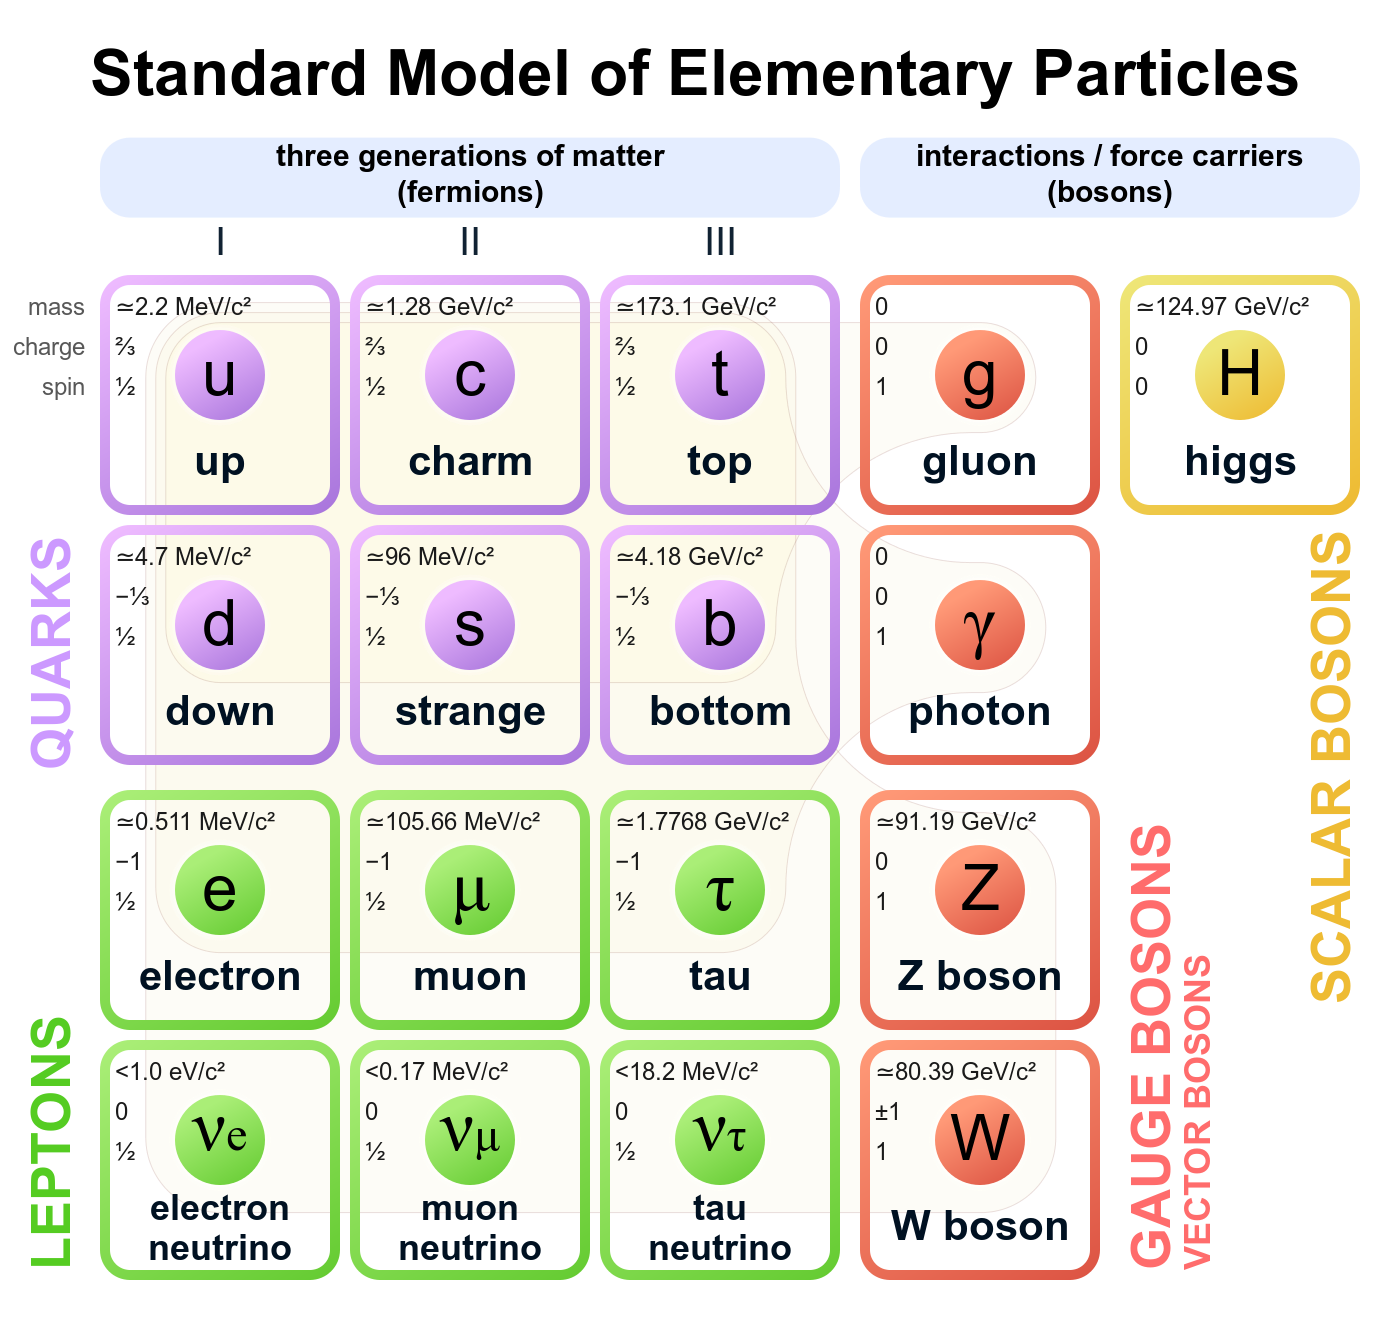
\includegraphics[width= 0.5 \columnwidth]{./sm.png}
	\caption{Elementary particles in standard model of particle physics with their mass, spin and charge.}
	\label{figure 1}
\end{figure}

\begin{figure}[H]
	\centering
	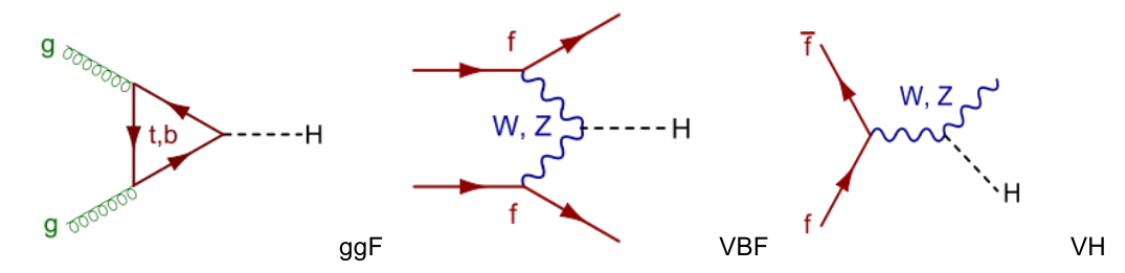
\includegraphics[width=\columnwidth]{./production_mode.png}
	\caption{Important production processes of Standard model Higgs boson ggF, VBF, VH in proton collisions.}
	\label{figure 2}
\end{figure}


\begin{figure}[H]
  \centering
   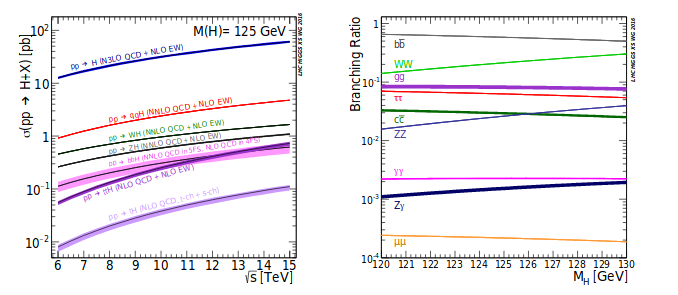
\includegraphics[scale=0.7]{./cd2.png}
  \caption{Standard model Higgs boson production cross section with center of mass energy and branching ratios for various decay channels \cite{Tanabashi:2018oca}.}
   \label{figure 3}
\end{figure}

\clearpage

 \newpage

The Standard Model (SM) of particle physics has successfully described most of the experimental data till now but a very large 
number of free-parameters and the fine tuning related to these parameters suggest new physics beyond SM. There are lot of specific 
BSM theories and most of these models involve new heavy particles. In order to identify which new physics lies beyond the 
electroweak (EW) scale, the new parameters  of such theories may be constrained by the actual low energy experiments. \\ 
%The fine tunings related to the Higgs mass and the free parameters in SM suggests new physics beyond Standard model (BSM). 

Until the 90's the existence of almost all the particles of the SM were confirmed except the top quark and the Higgs boson. 
These had eluded previous experiments due to difficulties in the production or reconstruction of its decays. The top quark was 
discovered in 1995 in the Tevatron collider of the Fermilab laboratory, this proton collider operated with a center of mass 
energy of 1.8 TeV untill 2010. The LHC collider at the CERN laboratory in Geneva, Switzerland, began its operations in 2010 
colliding protons at 7 TeV increasing the colliding energies to 8 and 13 TeV in the subsequent years. The Compact Muon Solenoid (CMS) is based on the Large Hadron Collider (LHC). It is designed to detect particles known as muons very accurately. In 2012, the ATLAS and CMS collaborations, with detectors at two points where the protons collide in the LHC, announced the discovery of a new boson with a mass of 125 GeV. So far, all measurements of the properties of this boson are consistent with those of the Higgs boson of the Standard Model (SM). \\

The CMS detector has the form of a cylindrical onion, with several concentric layers of components. Needed a powerful magnet to bend charged particles as they move away from the point of collision to identify the charge of the particles to bend them in opposite directions and measure momentum. A silicon tracker, made of about 75 
million electronic sensors arranged in concentric layers, identifies the tracks taken by these charged particles bent with very high precision \cite{Chatrchyan:2008aa}. The muons are detected by special subdetectors placed outside to detect them once they have crossed the solenoid as shown in Figure~\ref{figure5}.


LHC during the first run in 2011 and 2012 reached a peak instantaneous luminosity of 7.7 $\times$ $10^{33}$ $cm^{-2}s^{-1}$ which was more than 75$\%$ of its design luminosity and delivered an integrated luminosity of about 25 $fb^{-1}$ to each ATLAS and CMS. The luminosity delivered by the LHC during Run 1 (2011-2012),  Run 2 (2015-2018), and the expected luminosity for Run 3 and HL-LHC is shown in Figure 5. 

\clearpage
  \begin{figure}[H]
    \centering
    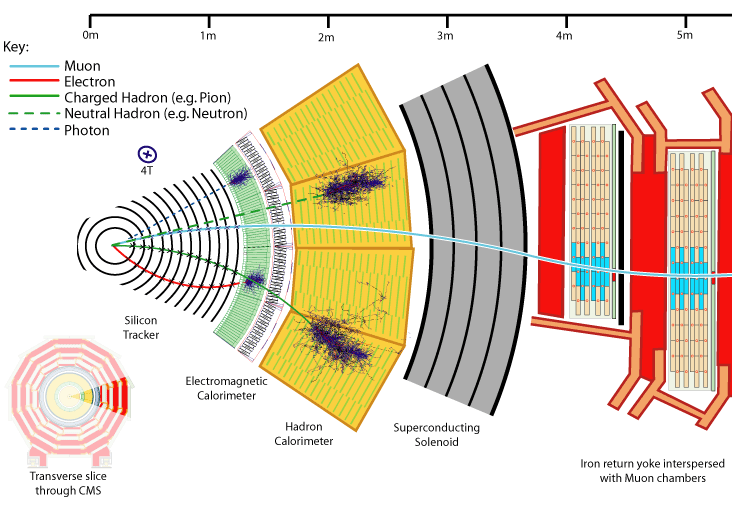
\includegraphics[width=0.6\columnwidth]{./cms12.png}
    \caption{Transverse view of the CMS detector showing the silicon tracker, electromagnetic calorimeter, hadron calorimeter, superconducting solenoid and muon chambers \cite{Chatrchyan:2008aa}.}
    \label{figure5}
  \end{figure}
  
  \begin{figure}[H]
    \centering
    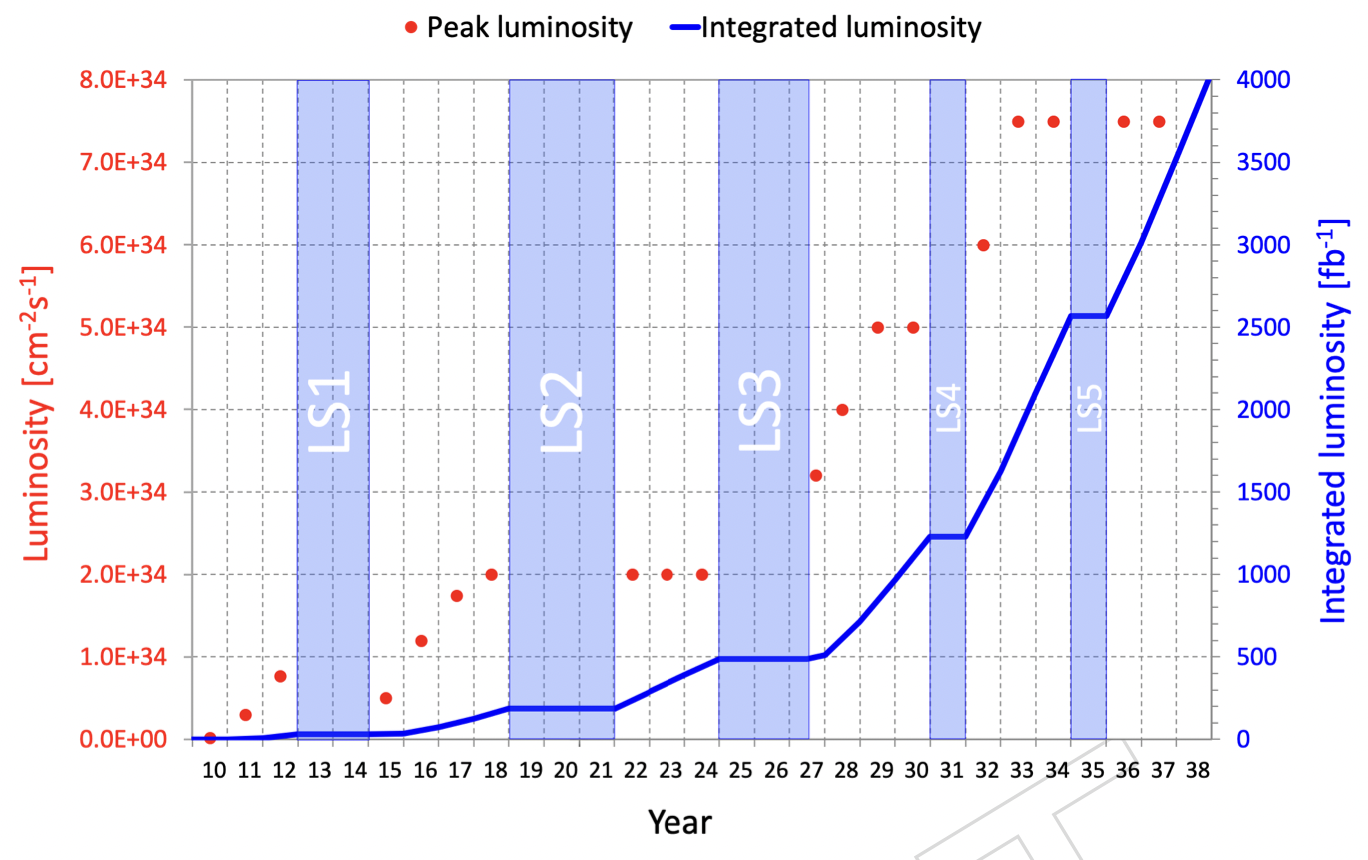
\includegraphics[width=0.9\columnwidth]{./HLLHCLumi.png}
    \caption{Projected performance of the LHC until 2038, which shows the preliminary dates for prolonged stops (LS) of the LHC and luminosities. Points show instantaneous luminosity while the line shows luminosity accumulated \cite{collaborations2019report}.}
    \label{figure6}
  \end{figure}


  
\clearpage
\section{PROPOSAL}
\onehalfspacing In this project, it is proposed to search for the decays of the Higgs boson to pairs of $J/\psi$ or $\Upsilon$ in the CMS detector based at the Large Hadron Collider of the CERN laboratory. For these studies the data of the LHC Run 2 (2015-2018) will be used corresponding to an integrated luminosity of about 150 fb$^{-1}$, this is 4 times larger than the dataset used for current results. Previously CMS has carried out studies with the data from 2017 ~\cite{2019134811} corresponding to 37.5 fb$^{-1}$ and ATLAS in 2012 ~\cite{PhysRevLett.114.121801} corresponding to 20.3 fb$^{-1}$.
    
\onehalfspacing We also propose to work on the luminosity measurement for the new LHC Run 3 which has just started in the year 2022. The measurement of the integrated luminosity is essential for many physics studies at CMS.

\section{GENERAL OBJECTIVE}
\onehalfspacing There is currently a great enigma in physics since we know that ordinary matter comprises only $5\%$ of the universe, another $27\%$ includes Dark matter and the rest $68\%$ is Dark energy.
Understanding the production of the Higgs boson, as well as its decays are an important part of the physics program of CERN laboratory experiments to verify the Standard Model and look for new particles. Through this project we will investigate the decay of the Higgs boson to pairs of $J/\psi$ or $\Upsilon$ in proton-proton collisions with the CMS experiment at the LHC. An observation of such decay  with this sample would indicate the presence of physics beyond the standard model. The decay to pairs of $J/\psi$ or $\Upsilon$ is expected to be extremely small, below  current detection limitations. 

\section{HYPOTHESIS}
\onehalfspacing With the CMS search mentioned above using 2017 data, an upper limit of $1.8 \times 10^{-3}$ was obtained in the $J/\psi$ pair while in the $\Upsilon$ pair channel, the limit was $1.4 \times 10^{-3}$. With this project we propose to incorporate the full Run 2 dataset corresponding to 150 fb$^{-1}$. A factor of 4 increase in number of collision events will improve the limits by a factor of approximately 2 due to the nature of statistical uncertainties. 


\section{SPECIFIC OBJECTIVES}

\onehalfspacing 
In order to complete a journal publication of this search the following are needed:
\begin{itemize}
\item Simulation of the signal events using Monte Carlo generators which implement the theoretical model.
\item Implementation of event reconstruction and selection algorithms which select high quality signal events and reduce the background events to a minimum.
\item Studies of lepton algorithms which improve the background rejection.
\item Reconstruction of $J/\psi$ and $\Upsilon$ with two muons ~\cite{Khachatryan_2014,Sirunyan_2018}.
\item Due to the small signal over background ratio, a multi-variate algorithm may be employed which combines different event variables and exploits the correlations to construct a final discriminant. This algorithm must be trained using simulated signal and background events.
\item A model for the observed data must be constructed from the known background processes. 
\item An fitting algorithm is developed that adjusts the model to the observed data distribution and incorporates several systematic uncertainties due to differences between simulation and real data. The signal strength observed from the statistical analysis must be interpreted as evidence of a signal or in the absence as a limit. 
\end{itemize}

In addition to the above objectives, members of the CMS collaboration are expected to participate in the detector operation and upgrade activities (or service work). During shut-down periods, these activities include testing and installation of new detectors.The luminosity data of run 3 will be studied and a luminosity measurement is planned for Run 3. For Run 2 we have these results ~\cite{CMS_PAS_LUM_17_004,CMS_PAS_LUM_18_002}.

\section{METHODOLOGY}

\onehalfspacing Accelerating the protons to extremely high energies and causing them to collide at high rates in order to produce rare but interesting events is the work of a separate accelerator group.
However, the members of the CMS collaboration must monitor the quality and rate of proton collisions at the interaction point at the center of the detector in order to collect a high quality dataset which can be stored for many years to do analysis.
Calibration and maintenance of all parts of the detector is necessary in order to achieve close to $100\%$ particle detection efficiency and noise levels to a minimum. This work is achieved by participating in the detector operation groups and performing data acquisition shifts during run time.  
Presence at CERN or at a remote control center like Fermilab is required in order to perform these activities. 

The reconstruction and selection of signal events is studied using the \textsc{MadGraph}~\cite{alwall2014automated} Monte Carlo generator which implements the theoretical model and predict the amount and distribution of events for a given LHC dataset.



A separate simulation of the detector is employed using \textsc{Geant}~\cite{agostinelli2003geant4} which simulates the trajectory of the stable particles, response and efficiency of each sensor in the CMS detector.
The information obtained from this chain is saved as raw data similar to the one obtained from the real experiment and is later reconstructed in the same way.

The event reconstruction is designed to capture the distinguishing features of the signal topology.
The event reconstruction begins with the identification of the different types of particles: photon, electrons, muons, taus, and jets.
Particle lists are formed for each kind using a general purpose event reconstruction software called \textsc{CMSSW}~\cite{Bayatian:922757} which is maintained by the collaboration and which includes basic calibration of the various particle energy and momenta.

The Tracker subdetector of CMS shown in Figure~\ref{figure5} is composed of silicon sensors which detect minimum ionizing charged particles coming from the interaction region. The Tracker consists of an inner Pixel detector with layers of pixel sensors and an outer Strip detector. The Pixel system consists of 66 Million pixels while the Strip system comprises of 9.6 Million strip sensors. The Tracker provides a precision measurement of the track curvature (momentum) and position at the interaction region.

Electrons are reconstructed from clusters of energy in the Electromagnetic calorimeter (ECAL). The ECAL is made of rectangular transparent crystals which cause a shower of secondary photons and electrons. The energy deposited in the crystal is read out and determines the energy of the primary electron. The cluster must match to a track in the Tracker subdetector. Photons are similar to electrons, but a track must not be matched in this case.

Muons are identified by tracks which exit the inner subdetectors and cross the solenoid into the Muon chambers. Drift Tubes (DT's) in the barrel region or Cathode Strip Chambers (CSC's) in the forward region use ionizing gas to detect the passage of muon tracks.  The track in the Muon chambers is matched to the track in the Tracker to provide a measurement of the muon momentum.

Jets are reconstructed from energetic clusters found in both the ECAL and the Hadronic calorimeter (HCAL).
Pions, kaons, and other hadrons create showers of secondary particles in the dense metal plates of the HCAL, the ionization energy of secondary particles is read out with scintillating plastics interleaved with the metal plates.  
Jets originate at the interaction region from collisions of quarks and gluons which create showers of mesons and baryons (mainly pions).


Luminosity is one of the most important parameter for a particle accelerator. It is the measure of number of proton-proton collisions occurring in unit centimetre square area per second. The installation of the CMS Phase-1 pixel detector took place during the extended year-end technical stop of the LHC in 2016/2017. The CMS Phase-1 pixel detector consists of four concentric barrel layers anf three disks. The CMS Phase-1 pixel detector is built from 1856 segmented silicon sensor modules,
where 1184 modules are used in the barrel pixel detector (BPIX) and 672 modules are used for the forward disks (FPIX). Each module consists of a sensor with 160x416 pixels connected to 16 readout chips (ROCs).One of the systems used for measuring luminosity at CMS is a technique called Pixel Cluster Counting (PCC) method. The PCC method uses the rate of pixel clusters in the CMS pixel detector to provide an luminosity measurement.

A new data structure with the above particle reconstruction defines new  datasets (\textsc{CMSSW}) stored in computing centers around the world which are available to students and scientists at all research institutions.
These  datasets are processed using computing clusters which use high-performance computing systems, normally using HTCondor~\cite{HTCondor} to link the processing nodes, which allows hundreds of jobs to run at the same time by individual users and save the output in \textsc{Root} format \cite{brun2003root}.
In this processing, the particle lists are used to require certain event selections and filter out uninteresting events.


Due to the small signal over noise ratio in this search, a multivariate algorithm is trained to help separate signal events from background events. A typical algorithm used is the Boosted Decision Tree~\cite{hoecker2007tmva}, which takes as input several event variables related to the signal topology. The multivariate algorithm takes into account the correlations between the variables and combines the information into a single discriminant. 

A fit is applied using the \textsc{RooFit} software package~\cite{verkerke2008roofit} which constructs a model for the data consisting of the sum of the backgrounds and the signal simulations. Systematic uncertainties are incorporated as nuisance parameters using gaussian probability functions, these account for uncertaintes in the normalization and shapes of the background.
The signal strength extracted from this fit determines if there is any evidence for a signal. In the absence of a signal an upper limit is placed on the signal strength using the likelihood function and subsequently translated into a limit.



\section{EXPECTED RESULTS}
\onehalfspacing The results from this project include the following items:
\begin{itemize}
\item Becoming author of an international collaboration.
\item A leading contribution in one of the search for decays of the Higgs boson into pairs of $J/\psi$ or $\Upsilon$ using the data from the Run II of the LHC, resulting in a publication in a scientific journal.
\item Improve limits on the branching fraction of these decays channels.
\item Luminosity measurements for RUN3 data.
\item A presentation of a poster or a talk in one of the national conferences of the Division of Paticles and Fields of the Mexican Society of Physics or a presentation of a poster or a talk in an international physics conference.
\item An academic stay at a scientific center like CERN or Fermilab.
\end{itemize}


\cleardoublepage
\section{CALENDAR OF ACTIVITIES}
\onehalfspacing
\begin{itemize}
\setlength\itemsep{-0.5em}
\item {\bf Semester 1 (2022-2)}: 
  \SubItem{ Readings on Standard Model theory}
  \SubItem{ Basic Linux computing skills (\textsc{Bash, Emacs, Root})}
  \SubItem{ Initial planning of the analysis strategy}
  \SubItem{ Initial work on 2022 luminosity measurement}
\item {\bf Semester 2 (2023-1)}:
  \SubItem{ Course I on particle physics and/or particle detection and analysis}
  \SubItem{ Basic Linux computing skills (\textsc{Bash, Emacs, Root})}
  \SubItem{ Readings on SM and $J/\psi$ and $\Upsilon$ literature}
  \SubItem{ Computing accounts at CERN and Fermilab}
  \SubItem{ Studies of the $J/\psi$ and $\Upsilon$ event selections}
  \SubItem{ Work on 2022 luminosity measurement}
  \SubItem{ Possible summer stay at CERN or Fermilab}
\item {\bf Semester 3 (2023-2)}:
  \SubItem{ Course II on particle physics and/or particle detection and analysis}
  \SubItem{ Studies of the $J/\psi$ and $\Upsilon$ event selections}
  \SubItem{ Studies of the background processes}
  \SubItem{ Work on 2023 luminosity measurement}
\item {\bf Semester 4 (2024-1)}:
  \SubItem{ Studies of the $J/\psi$ and $\Upsilon$ event selections}
  \SubItem{ Development of a Multivariate algorithm for the event selections}
  \SubItem{ Studies of the $J/\psi$ and $\Upsilon$ background processes}
  \SubItem{ Development of the statistical model and signal extraction}
  \Subitem{ Work on 2023 luminosity measurement}
  \SubItem{ Possible summer stay at CERN or Fermilab}
\item {\bf Semester 5 (2024-2)}:
  \SubItem{ Studies of the $J/\psi$ and $\Upsilon$ event selections}
  \SubItem{ Development of a Multivariate algorithm for the event selections}
  \SubItem{ Studies of the $J/\psi$ and $\Upsilon$ background processes}
  \SubItem{ Development of the statistical model and signal extraction}
  \Subitem{ Work on 2024 luminosity measurement}
\item {\bf Semester 6 (2025-1)}:
  \SubItem{ Completion of the Higgs reconstruction and background estimation methods}
  \SubItem{ Development of software for the statistical analysis and interpretation of the results}
  \SubItem{ Review process of the results within the CMS collaboration}
\item {\bf Semester 7 (2025-2)}:
  \SubItem{ Completion of the analisis work}
  \SubItem{ Writing of the paper publication}
  \SubItem{ Presentation of poster or talk at national or international conference}
\item {\bf Semester 8 (2026-1)}:
  \SubItem{ Writing of the thesis}
  \SubItem{ Completion of the paper publication}
  
\end{itemize}




\cleardoublepage
\onehalfspacing
\bibliographystyle{unsrt}
\bibliography{paper}

\end{document}

